\subsection{Digital Topology}
\label{sec:digital-topology}

Digital images consist of arrays of cubes.
Each cube is either black or white.
Given a digital image, one would like 
a computer to to classify the image.
Operations toward image classification include
object counting, border following and computing 
the homology of objects \cite{kong_digital_1989}.
Decomposing a cubical complex into a simplicial complex
results in 24 times as many highest dimensional cells \cite{Kaczynski2003}.


The elements of two-dimensional digital images
are \EMPH{pixels} and the elements of a three-dimensional
digital image are called \EMPH{voxels}.
Each pixel can be associated with a point in a lattice.
Two points in the lattice are four-adjacent if
they are  distinct and differ in at most one of their
coordinates, they are eight-adjacent
if they distinct and each coordinate entry differs by at most one.
In three dimensions, two points
are 26-adjacent if they are distinct and each coordinate 
entry differs by at most one.

If a set of points $S$ lattice points cannot be
partitioned into two subsets that are not
$n$-adjacent is \EMPH{$n$-connected}.

Consider four vertices adjacent to a single vertex $v$.
If four-adjacency is used the four black points are disconnected,
but separate $v$ from the exterior, if eight-adjacency is used
the back points form a Jordan curve that does not separate
an interior. To resolve this matter, we use eight-adjacency
for the white vertices and four-adjacency for the black.
We make a similar choice in three-dimensions.

\begin{figure}[htb]
        \centering
        \begin{subfigure}[b]{0.35\textwidth}
        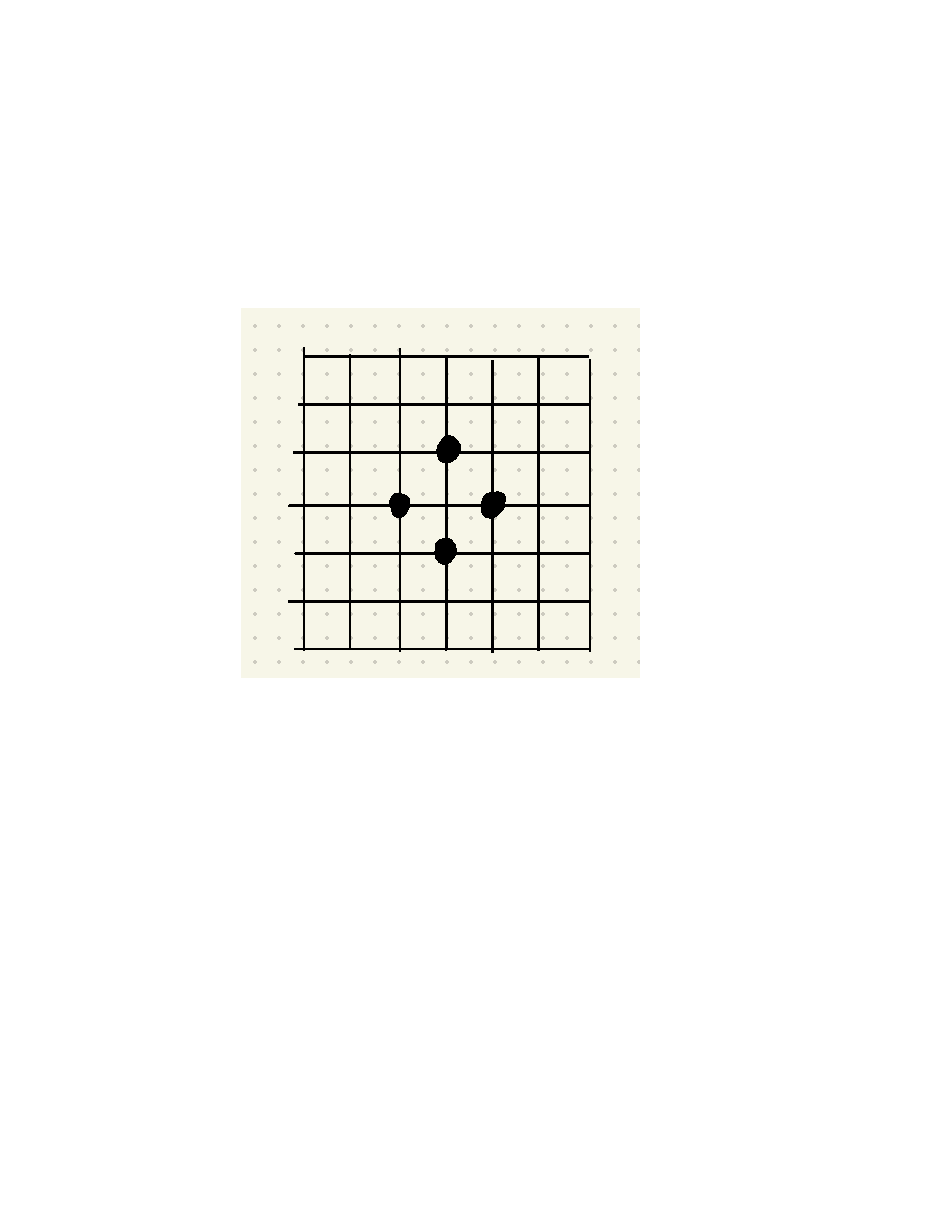
\includegraphics[width=\textwidth]{digital/paradox}
        \caption{}
          \label{fig:paradox}
        \end{subfigure}
          \hspace{.0cm}
         \begin{subfigure}[b]{0.40\textwidth}
        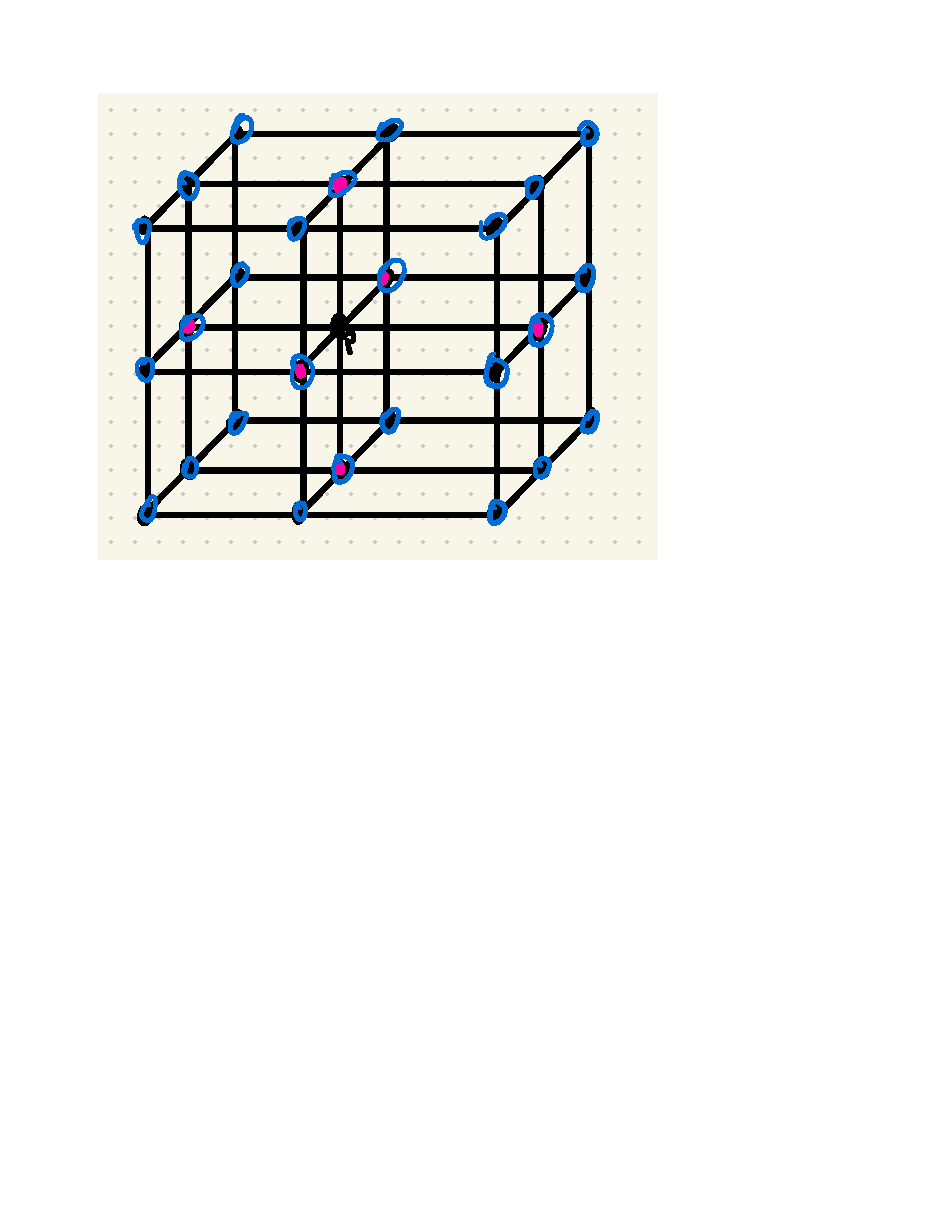
\includegraphics[width=\textwidth]{digital/6-26}
        \caption{}
        \label{fig:6-26}
        \end{subfigure}\\
		\caption{(a) Are the black points a closed curve? (b) In three-dimensions,
		the six neighbors of the vertex $p$ are in pink and the 26 neighbors are in
		blue. 
		\label{fig:adjacency}}
\end{figure}

A \EMPH{digital picture} is a quadruple $(V,m,n,B)$ where
$V=\R^2$ and $(m,n)=(4,8)$ or $V=\R^3$ and $(m,n)=(6,26)$
and $B$ is a subset of $V$. Elements of $B$ are black vertices
and elements not in $V$ are white.

In \cite{chen_digital_2010}, Chen and Rong an
algorithm to compute the homology groups of a three dimensional
digital object in $\R^3$. Their algorithm uses the Gauss-Bonnet theorem
and is linear in the size of the input.


We consider cubical spaces in $\R^3$ with $(6,26)$-connectivity,
where two points are adjacent  if their Euclidean distance is 1.
If $M$ is a closed, orientable digital surface, there are
six types of digital surface points, these are shown in \figref{surface-points}.

\begin{figure}[htb]
        \centering
        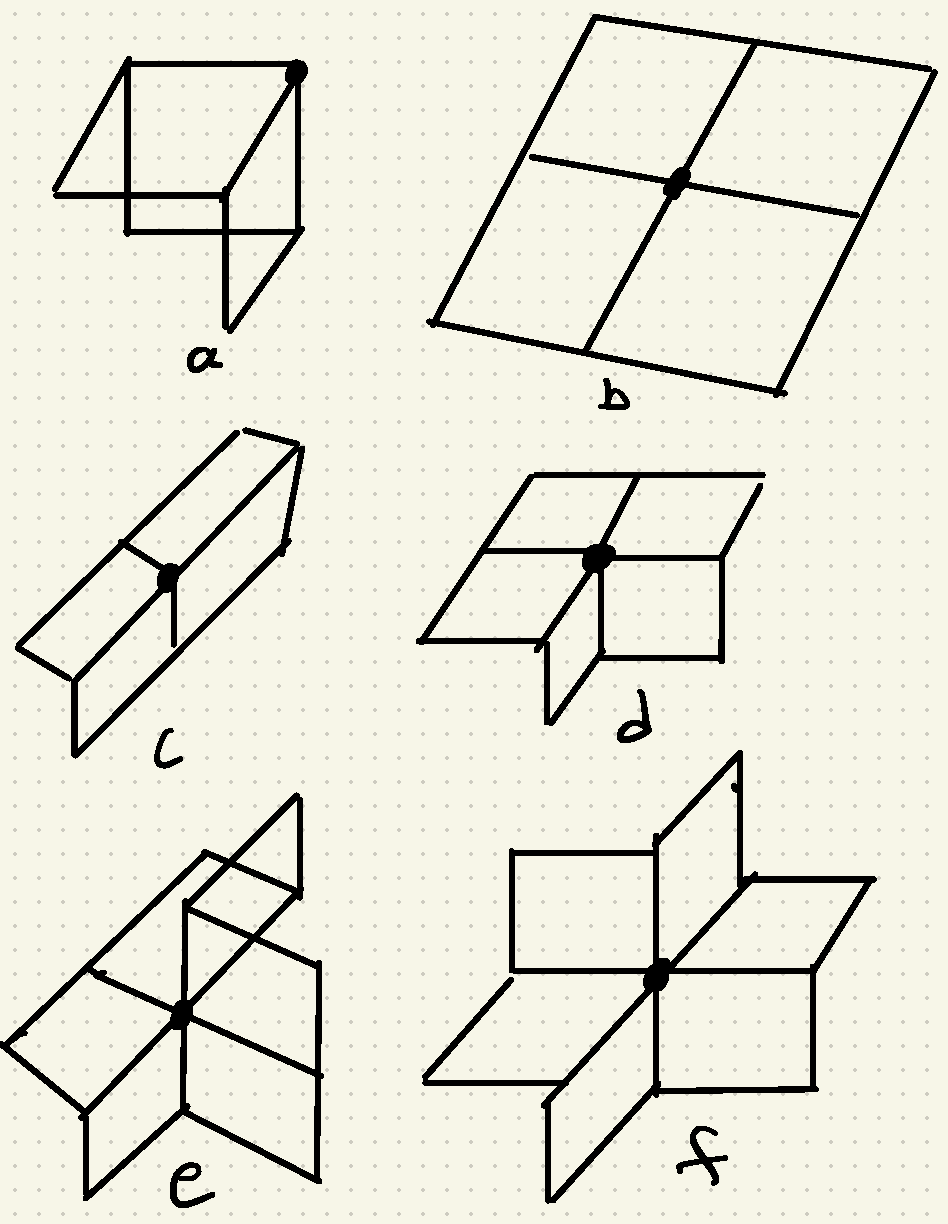
\includegraphics[width=.45\textwidth]{digital/surface-points}
		\caption{
		\label{fig:surface-points}}
\end{figure}

Let $M_i$ denote the set of digital points with $i$ neighbors and $K_i$
the curvature.
Then, by \eqnref{defect}, we have
\begin{enumerate}[(a)]
\item $K_3=\pi/2,$
\item $K_4=0,$
\item $K_5=-\pi/2,$
\item $K_6=-\pi.$
\end{enumerate}

For a closed two-manifold the is the boundary of a three-dimensional
digital image, the Gauss-Bonnet theorem implies
$$\sum_{i=3}^6K_i |M_i|=2(2-2g).$$
A linear time algorithm to compute the genus is the following.
Iterate through all points in $M$ and count the neighbors at each point
and keep track of $M_i$. Then use the above equation to  calculate the genus
using 
$$g=1+(|M_5|+2|M_6|-|M_3|)/8.$$